Dans un système ayant un seul PONE et un seul TARE (en plus du revendeur, du marché de gros et de l'AMI), le client demande une quantité d'énergie sans aucune contrainte particulière et sa demande est toute de suite satisfaite car le PONE produit exactement le type d'énergie demandé. Il y a donc achat (avec enregistrement de l'achat côté AMI) puis distribution au revendeur (en passant par le TARE).
Pour des soucis de simplicité au vue de notre modélisation, nous avons fais le choix
de requêter directement sur notre marché de gros qui est alimenté en permance et automatiquement par nos différents PONEs.
\\[1cm]
Lorsque le bouton "Scénario A" est actionné, nous requêtons notre marché de gros en lui demandant une énegie électrique quelque soit
son mode de production. Dans la requête du "Scénario A", nous passons dans la requête une demande qui est intiulée "Suivi commande". La demande d'énergie souhaitée est une énergie de type "électricité" avec un type d'extraction "Sans restriction" de plus nous passons une quantité égale à 1 pour être sur que celle-ci soit aboutie sans échec.

Il se peut que l'énergie envoyée soit du nucléaire ou du charbon ou encore eolien.

\begin{figure}[h]
    \centering
    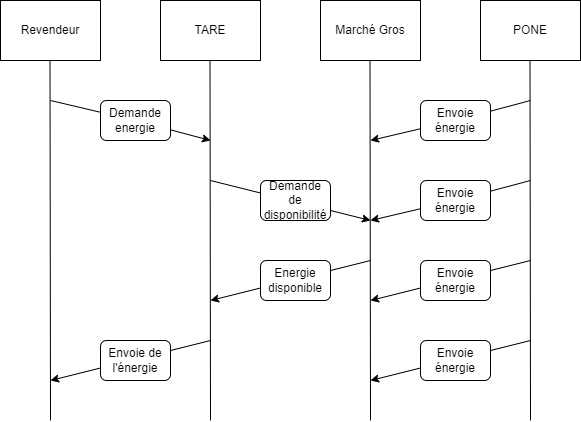
\includegraphics[width=100mm, height=73mm]{images/ScenarioA.png}
    \caption{Schéma du scénario A}
    \label{img:mesh21}
\end{figure}

\newpage
